\section{LTI-System}
Linear, zeitinvarianten System sind System $S$ mit Eingangssignal $x(t)$ und Ausgangssignal $y(t)$:
\begin{enumerate}[nosep]
	\item linear: $S\{a_1 \cdot x_1(t) + a_2 \cdot x_2(t)\} = a_1 \cdot S\{x_1(t)\} + a_2 \cdot S\{x_2(t)\}$ für $a,b \in \mathbb{R}$
	\item zeitinvariant: $S\{x(t)\} = y(t) \Rightarrow  S\{x(t + t_0)\} = S\{y(t + t_0)\}$ für $t_0 \in \mathbb{R}$
\end{enumerate}
~\\
Notation: $\underbrace{S}_\text{Operator}: x(t) \rightarrow y(t) = S\{x(t)\} = S[x](t)$

\section{Delta-Funktion}
Eine Delta-Funktion $\delta(x)$, auch Dirac-Stoss, modeliert ein unendlich Kurzen aber mit Fläche $1$ Stoss $\delta(t) = 0$ für $t \neq 0$. Damit lässt sich zB mit diskrete Werte rechnen.

\subsection{Eigenschaften}
\begin{align*}
	\int_{-\infty}^{\infty}\delta(t)dt &= 1 \\
	\int_{-\infty}^{\infty}\delta(t - t_0)f(t)dt &= f(t_0) \\
	\int_{-\infty}^{\infty}\left(\sum_{k=1}^{n}a_k\delta(t - t_k)f(t)\right)dt &= \sum_{k=1}^{n}a_kf(t)
\end{align*}

\section{Faltungsprodukt}
Mithilfe des Faltungsprodukt, oder auch Konvolution, kann zB von einem Dirac'schen Impuls die Systemantwort berechnet werden. Der Mathematische Operator $*$ wird dafür verwendet, um zwei Funktionen zu falten. Dabei wird die Funktion von links nach rechts durchgeschoben und die Fläche summiert.
\[
y(t) = (f * g)(t) = \int\limits_{-\infty}^{\infty}f(\tau)g(t - \tau)d\tau
\]

\noindent\textbf{Beispiel:} 
\[
f(t) = \begin{cases}
	t^2 - 4 & \text{für } \left|t\right| \lt 2 \\
	0 & \text{sonst}
\end{cases}
\quad \text{und} \quad 
g(t) = \begin{cases}
	1 & \text{für } -1 \lt t \lt 0 \\
	0 & \text{sonst}
\end{cases}
\]
Die Faltungsprodukt-Grenzen lassen sich über die Funktion und deren Grenzen bestimmen. Durch einsetzen der Funktionswerten mit entsprechendem $(\tau)$ bzw $(t-\tau)$ lässt sich ein $\tau(t)$-Diagram erstellen.
\begin{align*}
	f(\tau) = \tau^2 - 4 &\quad \xRightarrow[\left|t\right| \lt 2]{}& -2 \lt \tau \lt 2\\
	g(t-\tau)= 1 &\quad \xRightarrow[-1 \lt t \lt 0]{}& -1 \lt t-\tau \lt 0\\
	&												  & t \lt \tau \lt t +1
\end{align*}
\begin{center}
	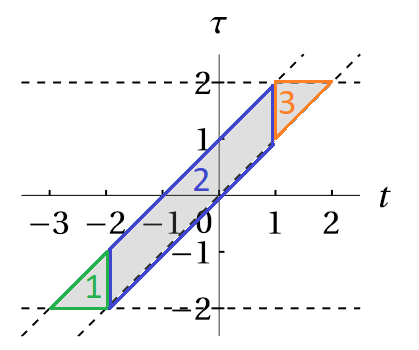
\includegraphics[width=0.4\columnwidth]{Images/faltprodukt}
\end{center}

\begin{align*}
	&& (f*t)(t) &= \int_{-\infty}^{\infty}f(\tau)g(t -\tau)d\tau \\
	&& t \leq -3       &: 0 \\
	(1) && -3 \lt t \lt -2 &: \int_{-2}^{t+1}(\tau^2 -4)\cdot 1d\tau = \frac{1}{3}t^3 + t^2 - 3t -9\\
	(2) && -2 \lt t \lt -1 &: \int_{-2}^{t+1}(\tau^2 -4)\cdot 1d\tau = t^2 + t - \frac{11}{3}\\
	(3) && 1 \lt t \lt 2   &: \int_{-2}^{t+1}(\tau^2 -4)\cdot 1d\tau = -\frac{1}{3}t^3 + 4t - \frac{16}{3}\\
	&& 2 \leq t &: 0 \\	
\end{align*}


\subsection{Eigenschaften}
	\begin{center}
		\begin{tabular}{l|l}
		Kommutativ & $(f * g)(t) = (g*f)(t)$ \\ \midrule
		Ausblendeigenschaft & $f(t)*\delta(t-t_0)=f(t-t_0)$
	\end{tabular}
\end{center}
